% ------------------------------------------------------------------------
% file `ad-complogic-report-exercise-5-solution-body.tex'
%
%     solution of type `exercise' with id `5'
%
% generated by the `solution' environment of the
%   `xsim' package v0.10 (2017/09/19)
% from source `ad-complogic-report' on 2017/11/26 on line 432
% ------------------------------------------------------------------------
^^I^^IОскільки для побудови функціональної схеми необхідно використати T-тригери, наведемо таблицю їх переходів~(табл.~\ref{tab:task-5-t-flipflop-excitation-table}). Побудуємо таблицю, що описує заданий автомат~(табл.~\ref{tab:task-5-automata-table}). Для цього пронумеруємо стани за принципом кодування Грея: $a_1$~— $00$, $a_2$~— $01$, $a_3$~— $11$.
^^I^^I
^^I^^I\begin{table}[!htbp]
^^I^^I\centering
^^I^^I^^I\begin{tabular}{ccc}
^^I^^I^^I^^I\toprule
^^I^^I^^I^^I^^I$Q_t$ & $Q_{t+1}$ & T\\
^^I^^I^^I^^I\midrule
^^I^^I^^I^^I^^I0     & 0         & 0\\
^^I^^I^^I^^I^^I1     & 1         & 0\\
^^I^^I^^I^^I^^I0     & 1         & 1\\
^^I^^I^^I^^I^^I1     & 0         & 1\\
^^I^^I^^I^^I\bottomrule
^^I^^I^^I\end{tabular}
^^I^^I\caption{Таблиця переходів T-тригера}
^^I^^I\label{tab:task-5-t-flipflop-excitation-table}
^^I^^I\end{table}
^^I^^I
^^I^^I\begin{table}[!htbp]
^^I^^I\centering
^^I^^I^^I\begin{tabular}{cccccccccc}
^^I^^I^^I^^I\toprule
^^I^^I^^I^^I^^I% Make the header 2-row with multicolumns T and T + 1
^^I^^I^^I^^I^^I\multicolumn{3}{c}{$t$} & \multicolumn{6}{c}{$t + 1$} \\
^^I^^I^^I^^I^^I\cmidrule(lr){1-3} \cmidrule(lr){4-9}
^^I^^I^^I^^I^^I$A_1$ & $A_2$ & $x_1$ & $A_1$ & $A_2$ & $y_1$ & $y_2$ & $T_1$ & $T_2$\\
^^I^^I^^I^^I\midrule
^^I^^I^^I^^I^^I$0$   & $0$   & —     & $0$   & $1$   & $0$   & $1$      & 0     & 1\\
^^I^^I^^I^^I^^I$0$   & $1$   & $0$   & $1$   & $1$   & $0$   & $0$      & 1     & 0\\
^^I^^I^^I^^I^^I$1$   & $1$   & $1$   & $0$   & $0$   & $0$   & $0$      & 1     & 1\\
^^I^^I^^I^^I^^I$1$   & $1$   & —     & $1$   & $0$   & $1$   & $0$      & 0     & 1\\
^^I^^I^^I^^I\bottomrule
^^I^^I^^I\end{tabular}
^^I^^I\caption{Таблиця заданого автомата}
^^I^^I\label{tab:task-5-automata-table}
^^I^^I\end{table}
^^I^^I
^^I^^IСкладемо та мінімізуємо функції, що описують залежності станів:
^^I^^I\begin{IEEEeqnarray*}{rCl}
^^I^^I^^IT_1 (A_1, A_2, x) &=& \neg{A_1} \land A_2 \lor A_2 \land x,\\
^^I^^I^^IT_2 (A_1, A_2, x) &=& \neg{A_1} \land \neg{A_2} \lor A_1 \land A_2.\\
^^I^^I^^Iy(A_1, A_2, x)    &=& A_1 \land \neg{x},\\
^^I^^I^^Iy(A_1, A_2, x)    &=& \neg{A_2}.\\
^^I^^I\end{IEEEeqnarray*}
^^I^^I
^^I^^IЗа мінімізованими функціями будуємо функціональну схему керуючого автомата~(рис.~\ref{fig:task-5-schematic}) в базисі, що складається з логічних елементів І, НЕ, АБО.
^^I^^I
^^I^^I\begin{figure}[!htbp]
^^I^^I\centering
^^I^^I^^I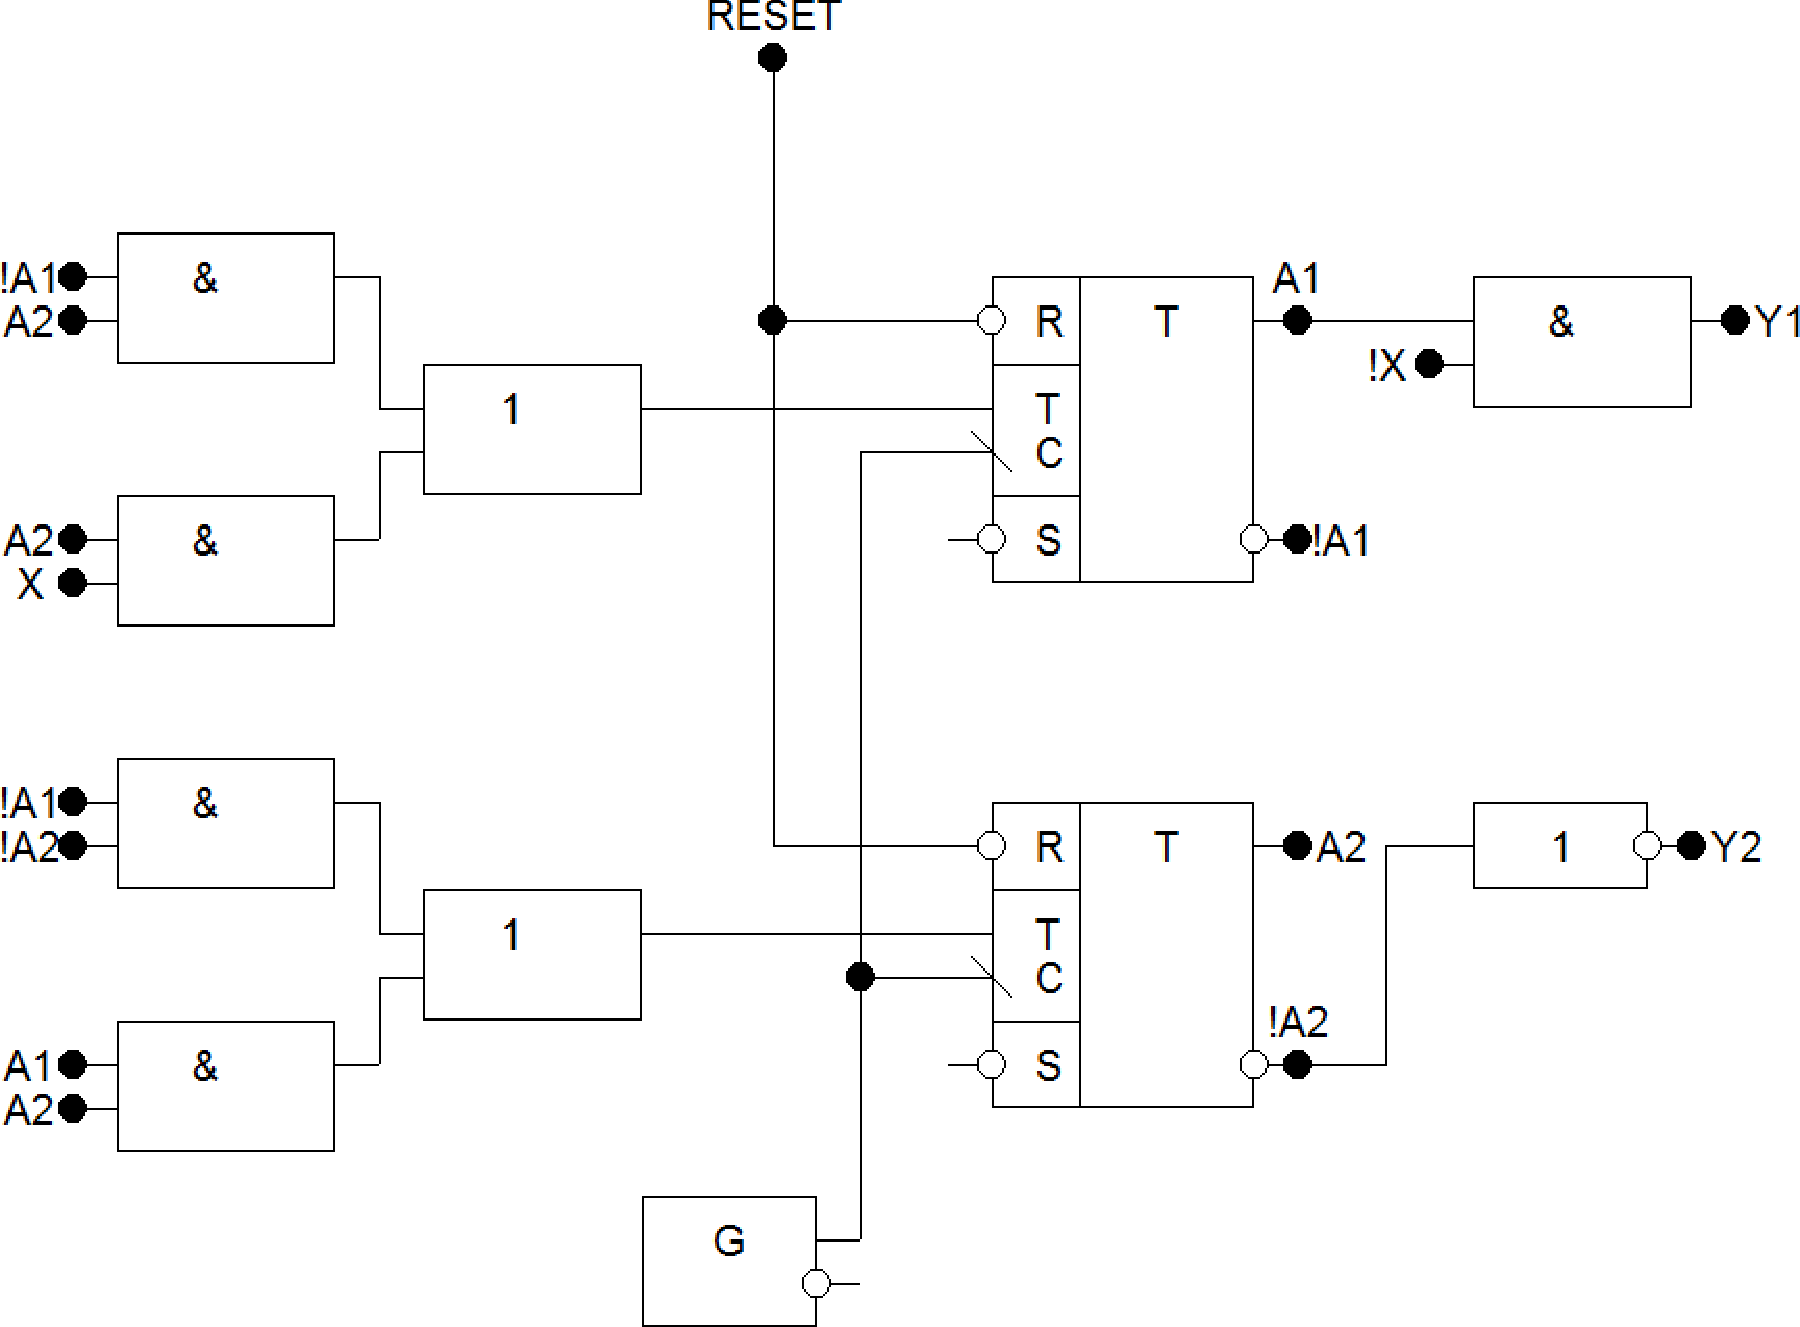
\includegraphics[height = 16\baselineskip]{../schematic-trimmed.pdf}
^^I^^I\caption{Функціональна схема керуючого автомата}
^^I^^I\label{fig:task-5-schematic}
^^I^^I\end{figure}
